\chapter{Cadyts}
\label{ch:cadyts}
% ##################################################################################################################

\hfill \textbf{Authors:} Kai Nagel, Michael Zilske, Gunnar Fl\"otter\"od

\begin{center} 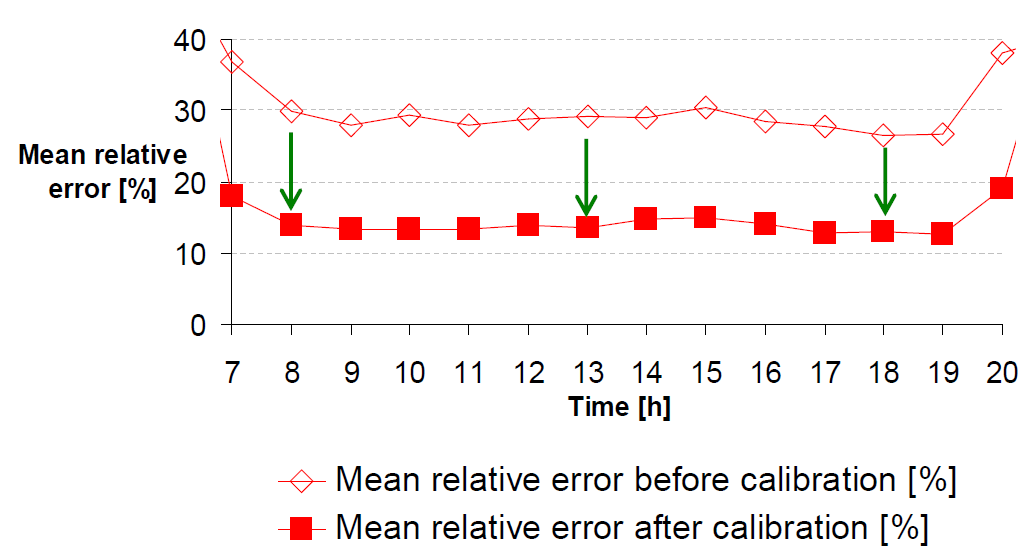
\includegraphics[width=0.5\textwidth, angle=0]{extending/figures/cadyts/cadyts} \end{center}

\createStandardInformation{cadytsIntegration}
{\lstinline{RunCadyts4CarExample} class}
{cadytsCar}
{\citet[][]{cadyts-manual, floetteroed-2010e, FloetteroedChenEtAl2011BehavioralCalibAndAnaNETS, Floetteroed2008PhD, Moyo2013PhD}}

% ##################################################################################################################

%\ah{adopted from \citet[][]{Floetteroed2009CadytsSTRC}. Please check, in particular copy rights of figure}
%\gunnar{Checked. -- Die Abbildung taucht in dem NETS paper gar nicht auf. Sollte so gesehen unproblematisch sein.}
%\ah{ok}

% ##################################################################################################################
\section{Introduction}

\gls{cadyts}\footnote{\url{http://people.kth.se/~gunnarfl/cadyts.html}}
---licensed under \gls{gplv3}---calibrates disaggregate travel demand models 
of \gls{dta} simulators from traffic counts and vehicle re-identification data. 
\gls{cadyts} is compatible with a broad class of \gls{dta} microsimulators,
into which it can be hooked through sparse interfaces.

As explained in formal terms in Chapter~\ref{ch:abta} and~\ref{ch:montecarlo}, 
\gls{dta} targets at consistency between a dynamic model of travel 
demand---in \gls{matsim} represented by the agents' plans---
and a dynamic model of network supply, capturing the spatiotemporal
evolution of network flows and congestion.

\gls{cadyts} adjusts the plan choice probabilities of all 
agents such that they result in simulated network conditions that are consistent with 
measured real-world data, while maintaining behavioral 
plausibility in terms of the underlying travel demand model. 
Within MATSim, the adjustment of plan choice probabilities is realized 
by adjusting the plan scores, as explained in the next section.

% ##################################################################################################################
\section{Adjusting Plans Utility}

In case of traffic counts being the empirical source, the plan-specific score corrections 
are composed of link- and time-additive terms $\Delta S_a(k)$ for each link $a$
and each calibration time step $k$ (often one hour). 
In case congestion is light and traffic counts are independently and normally distributed, 
these correction terms become 
%\cite[p.487]{FloetteroedChenEtAl2011BehavioralCalibAndAnaNETS}
%
\begin{equation}
\label{eq:cadyts:correction}
\Delta S_a(k) = \frac{y_a(k) - q_a(k)} {\sigma_a^2(k)}
\end{equation}
%
where $y_a(k)$ is the real-world measurement on link $a$ in time step $k$, 
$q_a(k)$ is its simulated counterpart, and $\sigma^2_a(k)$ is (an estimate of) 
the variance of the real measurement (assuming that its expected value 
coincides with the prediction $q_a(k)$ of a perfectly calibrated simulator).

The score correction of a given activity-travel plan of an agent is calculated as 
the sum of all $\Delta S_a(k)$ for which it is foreseeable that following that plan 
implies entering link $a$ within time step $k$. 
%\citep{FloetteroedChenEtAl2011BehavioralCalibAndAnaNETS}.
With this, the \textit{a posteriori} choice probability of plan $i$ of agent $n$ given
the count data ${\bf y} = \{y_a(k)\}$ becomes
%
\begin{equation}
P_n(i\mid{\bf y}) \sim 
\exp\left(S_n(i)+ \sum_{ak\in_{}i} \Delta S_a(k) \right)
\,\,=\,\,
\exp\left(S_n(i)+ \sum_{ak\in_{}i} \frac{y_a(k) - q_a(k)} {\sigma_a^2(k)} \right)
\label{eq:cadyts:selection}
\end{equation}
where $S_n(i)$ is the \textit{a priori} score of a plan $i$ of agent $n$ as 
calculated for example with Equation~(\ref{eq:matsimUTF}) and $ak\in i$ reads as
``following plan $i$ implies entering link $a$ in time step $k$''.

Intuitively, if the simulation value $q_a(k)$ is smaller than the real measurement 
$y_a(k)$, then an increase in score and thus an increase in choice 
probability results. 
$\sigma^2_a(k)$ denotes how much one should trust that specific measurement
---a large variance $\sigma^2_a(k)$ implies a low trust level that takes effect through
an accordingly large denominator in the corresponding addend of the score correction.

\citet[][]{floetteroed-2010e} is the key methodological reference on \gls{cadyts}.
It derives the calibration approach from a Bayesian argument and provides
further technical information, such as a more general functional form of the utility
correction in Equation~(\ref{eq:cadyts:correction}) that also applies in the presence
of congestion. A more lightweight presentation is 
\citet[][]{FloetteroedChenEtAl2011BehavioralCalibAndAnaNETS}, where the above
formulas are also discussed in somewhat greater detail.

% ##################################################################################################################
\section{Hooking Cadyts Into MATSim}
Hooking \gls{cadyts} into \gls{matsim} is based on the following operations.
\begin{enumerate}\styleEnumerate
\item Initialization: When the calibration is started, it needs to be provided with all available 
traffic counts and some further parameters. 
For this, the \gls{cadyts} function \lstinline|void addMeasurement(...)| is called once for every 
measurement before the simulation starts. It registers a measurement of a certain type, which 
has been observed on a certain link.
\item Iterations: The calibration is run jointly with the simulation until (calibrated) 
stationary conditions are reached.
	\begin{itemize}[(a)]\styleItemize
	\item Demand simulation: The calibration needs an access point in the simulation in order 
	to affect the plan choice. There are various ways to realize this, depending on the concrete 
	simulator.	
	\gunnar{Trifft Folgendes f\"ur MATSim zu? Ich habe diesen Funktionsaufruf aus der
	CadytsScoring-Klasse herausgefischt, bin mir aber nicht sicher, wie das auf der MATSim-Seite
	zusammenspielt.}
	\ah{m.E. geschieht genau das in \lstinline|org.matsim.contrib.cadyts.general.CadytsPlanChanger.selectPlan(...)|}
	Before a \gls{matsim} agent chooses a plan, he or she asks the calibration through the 
	\gls{cadyts} function
	\lstinline|double calcLinearPlanEffect(Plan plan)| for the score offsets for
	all of its plans.
	The agent then chooses a plan based on accordingly modified scores.
	\item Supply simulation: The calibration needs to observe the simulated network conditions 
	in order to evaluate their deviation from the real traffic counts.
	For this, the \gls{cadyts} function \lstinline|void afterNetworkLoading(SimResults simResults)| 
	is called once after each network loading. It passes a container object to the calibration that 
	provides information about the results of the most recent network loading, in particular about 
	the simulated flows at the measurement locations.
	\end{itemize}
\end{enumerate}

% ##################################################################################################################
\section{Applications}
\gls{cadyts} has been successfully applied in studies such as % FloetteroedEtAl2009IatbrCalibration, 
\citet[][]{ZiemkeNagelBhat2014IntegratingCemdapMatsimTransferabilityVSPWP, ZilskeNagelPhoneTracesAndCadyts, FloetteroedChenEtAl2011BehavioralCalibAndAnaNETS}. 
Its efficiency is evident in the Zürich scenario results as shown in \citet[][Slide~8]{FloetteroedEtAl_unpub_MATSimUserMeeting_2011}, 
reproduced in Figure~\ref{fig:cadyts}.

\createfigure%
{Zürich case study results: mean relative error in link volumes}%
{Zürich case study results: mean relative error in link volumes}%
{\label{fig:cadyts}}%
{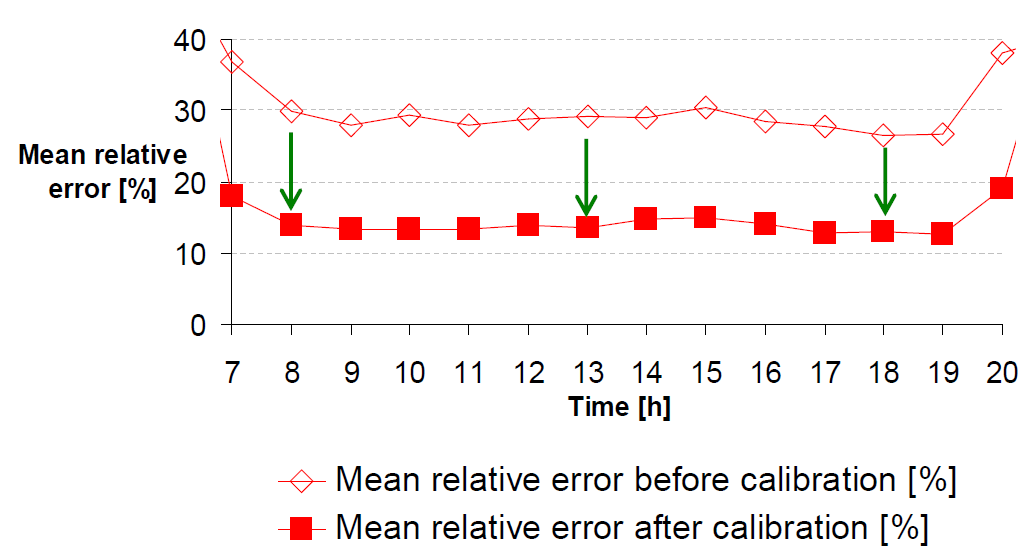
\includegraphics[width=0.8\textwidth, angle=0]{extending/figures/cadyts/cadyts}}%
{\citet[][Slide~8]{FloetteroedEtAl_unpub_MATSimUserMeeting_2011}}

% ##################################################################################################################
% Local Variables:
% mode: latex
% mode: reftex
% mode: visual-line
% TeX-master: "../../main"
% comment-padding: 1
% fill-column: 9999
% End: 
